%-----------------------------------------------------------------------------
%
%               Template for sigplanconf LaTeX Class
%
% Name:         sigplanconf-template.tex
%
% Purpose:      A template for sigplanconf.cls, which is a LaTeX 2e class
%               file for SIGPLAN conference proceedings.
%
% Guide:        Refer to "Author's Guide to the ACM SIGPLAN Class,"
%               sigplanconf-guide.pdf
%
% Author:       Paul C. Anagnostopoulos
%               Windfall Software
%               978 371-2316
%               paul@windfall.com
%
% Created:      15 February 2005
%
%-----------------------------------------------------------------------------


\documentclass{sigplanconf}

% The following \documentclass options may be useful:

% preprint      Remove this option only once the paper is in final form.
% 10pt          To set in 10-point type instead of 9-point.
% 11pt          To set in 11-point type instead of 9-point.
% authoryear    To obtain author/year citation style instead of numeric.

\usepackage[ruled,vlined]{algorithm2e}
\usepackage{amsmath}
\usepackage{amsthm}
\usepackage{bm}
\usepackage{tikz}
\usetikzlibrary{decorations.markings}
\usetikzlibrary{positioning}
\tikzstyle{vertex}=[circle, draw, inner sep=0pt, minimum size=6pt]

\begin{document}

\special{papersize=8.5in,11in}
\setlength{\pdfpageheight}{\paperheight}
\setlength{\pdfpagewidth}{\paperwidth}

\conferenceinfo{CONF 'yy}{Month d--d, 20yy, City, ST, Country}
\copyrightyear{20yy}
\copyrightdata{978-1-nnnn-nnnn-n/yy/mm}
\doi{nnnnnnn.nnnnnnn}

% Uncomment one of the following two, if you are not going for the
% traditional copyright transfer agreement.

%\exclusivelicense                % ACM gets exclusive license to publish,
                                  % you retain copyright

%\permissiontopublish             % ACM gets nonexclusive license to publish
                                  % (paid open-access papers,
                                  % short abstracts)

\titlebanner{banner above paper title}        % These are ignored unless
\preprintfooter{short description of paper}   % 'preprint' option specified.

\title{Elizabeth Scott Explained}
\subtitle{Parsing from Earley Recognisers}

\authorinfo{Zoe Wheeler}
           {University of Texas at Austin}
           {zoe.donnellon.wheeler@gmail.com}
\authorinfo{Walter Xia}
           {University of Texas at Austin}
           {swilery@utexas.edu}

\maketitle

\begin{abstract}
Earley's Algorithm is able to recognize general context-free grammars in $O(n^3)$, where $n$ is the size of the string to be recognized. However, there are times in which we want more than just a yes or no answer. There are times in which we want an actual parse tree, and for ambiguous grammars, there are times in which we want all possible parse trees. Fortunately, there is a paper by Dr. Elizabeth Scott, \cite{scott}, that presents a technique to produce a data structure known as a Shared Packed Parse Forest (SPPF), able to represent even an infinite number of parse trees. Unfortunately this paper is poorly written, making it very difficult to understand. Our paper is a re-explanation of Scott's techniques. It is agreed by many that Earley's Algorithm is also difficult to understand. Fortunately, there exists a data structure due to Dr. Gianfranco Bilardi and Dr. Keshav Pingali, \cite{bilardi-pingali}, known as Grammar Flow Graphs (GFGs) that significantly ease the understanding of the algorithm by reformulating parsing problems as path problems in a graph. Our technique will use GFGs.
\end{abstract}

\category{F.7.2}{Semantics and Reasoning}{Program Reasoning--Parsing}

% general terms are not compulsory anymore,
% you may leave them out
\terms
Context-Free Languages, Cubic Generalized Parsing, Earley Parsing 

\keywords
Earley Sets, Grammar Flow Graphs, Non-Deterministic Finite Automaton, Shared Packed Parse Forest

\section{Introduction}
It is important here for us to distinguish between recognisers and parsers for a grammar. Recognizers determine whether or not a string is part of a language defined by a grammar whereas parsers construct parse trees that reveal \textit{how} a string satisfies the syntax dictated by a grammar. For about the past five decades, there already exist general recognizers like Cocke-Younger-Kasami (CYK) and Earley's Algorithms that run cubic relative to the size of the string to be recognized. Alternatively, Generalized LR (GLR) is an algorithm that produces parsers but has the very undesirable property that it is unbounded. Dr. Elizabeth Scott extended the Earley Recogniser into a parser that is able run in cubic space and time, \cite{scott}. The challenge was to successfully apply the parser to ambiguous grammars that produces multiple, perhaps infinite, parse trees for a string in the grammar. Note that simply disallowing ambiguous grammars is not a solution since there exists grammars that are intrinsically ambiguous. The solution she used was a representation known as a Shared Packed Parse Forest (SPPF), which is in essence a Directed Acyclic Graph (DAG).

Earley's Algorithm is a highly complex algorithm. To dramatically simplify its understanding, we view it from the perspective of Grammar Flow Graphs (GFGs) that restructure parsing as finding certain paths within the graph, \cite{bilardi-pingali}. For those of you familiar with automata theory, GFGs play the same role for context-free grammars as finite-state automota play for regular grammars. The rest of the paper is organized as follows:
\begin{itemize}
\item Section 2 will introduce GFGs
\item Section 3 will introduce Earley's Algorithm using GFGs
\item Section 4 will introduce SPPFs
\item Section 5 will introduce Dr. Scott's Algorithm for producing SPPFs
\item Section 6 will discuss our implementation
\item Section 7 will conclude with our results and future work
\end{itemize}

\section{Grammar Flow Graphs}
Let us begin with the standard definition of a context-free grammar.

\textit{Definition:} A \textit{context-free grammar}, \textit{CFG}, is a tuple $(N, T, P, S)$, where, \cite{bilardi-pingali}:
\begin{itemize}
\item[$\triangleright$] $N$ is a finite set of elements called \textit{nonterminals}, 
\item[$\triangleright$] $T$ is a finite set of elements called \textit{terminals}, 
\item[$\triangleright$] $P\subseteq{N\times{(N\cup{T}}})^*$ is the set of \textit{productions} that map nonterminals to a sequence of nonterminals or terminals, and 
\item[$\triangleright$] $S\in{N}$ is the unique \textit{start symbol} that appears once on the left-hand side of a single production.
\end{itemize}

An example of a grammar is the following, where $|$ signifies or:
\begin{align*}
S&\longrightarrow{N \: t \: | \: t \: N} \\
N&\longrightarrow{t \: t}
\end{align*}

Now we are in a position to introduce the GFG.

\textit{Definition:} Let $CFG = (N, T, P, S)$ be a context-free grammar and let $\epsilon$ denote the empty string. The \textit{grammar flow graph (GFG)} of $CFG$, $GFG(CFG) = (V(CGF), G(CFG))$, is the smalled directed graph that has the following properties, \cite{bilardi-pingali}:
\begin{itemize}
\item[$\triangleright$] For each nonterminal $M\in{N}$, there exist $(\bullet{M})$,$(M\bullet){\in{V(CFG)}}$ called \textit{start nodes} and \textit{end nodes} respectively,
\item[$\triangleright$] For each production $(M\longrightarrow{\epsilon})\in{P}$, there exists $(M\longrightarrow{\bullet})\in{V(CFG)}$ and $(\bullet{M}, M\longrightarrow{\bullet}),(M\longrightarrow{\bullet}, M\bullet)\in{E(CFG)}$,
\item[$\triangleright$] For each production $(M\longrightarrow{q_1q_2\dots{q_r}})$ where $q_i \neq \epsilon$:
\begin{itemize}
\item[$\diamond$] $(M\longrightarrow{\bullet{q_1q_2\dots{q_r}}}), (M\longrightarrow{q_1\bullet{q_2\dots{q_r}}}), \dots, (M\longrightarrow{q_1q_2...q_r\bullet})\in{V(CFG)}$, where the first node is called an \textit{entry node} and the last node is called an \textit{exit node},
\item[$\diamond$] $(\bullet{M}, M\longrightarrow{\bullet{q_1q_2\dots{q_r}}}), (M\longrightarrow{q_1q_2\dots{q_r\bullet}}, M\bullet)\in{E(CFG)}$ called \textit{entry edges} and \textit{exit edges} respectively,
\item[$\diamond$] For each $t\in{T}$, $(M\longrightarrow{\dots{\bullet{t\dots}}}, M\longrightarrow{\dots{t\bullet{\dots}}})\in{E(CFG)}$ called \textit{scan edges} labeled $t$, where $(M\longrightarrow{\dots{\bullet{t\dots}}})$ is called a \textit{scan node}, and
\item[$\diamond$] For each $K\in{N}$, $(M\longrightarrow{\dots{\bullet{K\dots}}}, \bullet{K})$, $(K\bullet, M\longrightarrow{\dots{K\bullet{\dots}}})$ called \textit{call edges} and \textit{return edges} respectively, where $(M\longrightarrow{\dots{\bullet{K\dots}}})$ is called a \textit{call node} that is matched with the \textit{return node} $(M\longrightarrow{\dots{K\bullet{\dots}}})$, and
\end{itemize}
\item[$\triangleright$] Edges not scan edges are labeled $\epsilon$.
\end{itemize}
\begin{figure}
\begin{center}
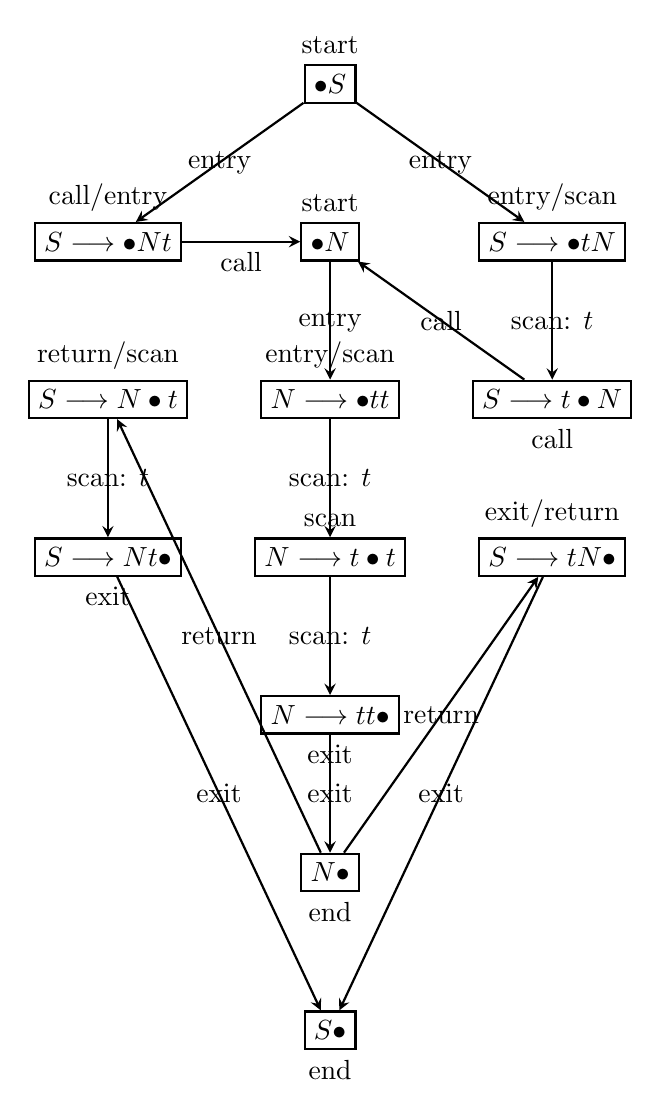
\begin{tikzpicture}[->,>=stealth,node distance = 1.5cm,thick]
\tikzstyle{v}=[rectangle,minimum size=1mm,draw,thick]
\node[v, label=start]	(dotS)  					   		{$\bullet{S}$};
\node[v, label=start] 	(dotN)  	[below = of dotS]		{$\bullet{N}$};
\node[v, label=entry/scan] 	(dottt)  	[below = of dotN]		{$N\longrightarrow{\bullet{tt}}$};
\node[v, label=scan] 	(tdott)  	[below = of dottt]		{$N\longrightarrow{t\bullet{t}}$};
\node[v, label={[below = 0.5cm]:exit}] 	(ttdot)  	[below = of tdott]		{$N\longrightarrow{tt\bullet}$};
\node[v, label={[below = 0.5cm]:end}] 	(Ndot)  	[below = of ttdot]		{$N\bullet$};
\node[v, label={[below = 0.5cm]:end}] 	(Sdot)  	[below = of Ndot]		{$S\bullet$};
\node[v, label=call/entry] 	(dotNt)		[left = of dotN]		{$S\longrightarrow{\bullet{Nt}}$};
\node[v, label=return/scan] 	(Ndott)  	[below = of dotNt]		{$S\longrightarrow{N\bullet{t}}$};
\node[v, label={[below = 0.5cm]:exit}] 	(Ntdot)  	[below = of Ndott]		{$S\longrightarrow{Nt\bullet}$};
\node[v, label=entry/scan] 	(dottN)  	[right = of dotN]		{$S\longrightarrow{\bullet{tN}}$};
\node[v, label={[below = 0.5cm]:call}] 	(tdotN)  	[below = of dottN]		{$S\longrightarrow{t\bullet{N}}$};
\node[v, label=exit/return] 	(tNdot)  	[below = of tdotN]		{$S\longrightarrow{tN\bullet}$};
\path(dotS)		edge	node			{entry}		(dotNt)
	 (dotS)		edge	node			{entry}		(dottN)
	 (dotNt)	edge	node[below]			{call}		(dotN)
	 (tdotN)	edge	node			{call}		(dotN)
	 (dotN)		edge	node			{entry}		(dottt)
	 (dottt)	edge	node		{scan: $t$}	(tdott)
	 (tdott)	edge	node		{scan: $t$}	(ttdot)
	 (ttdot)	edge	node			{exit}		(Ndot)
	 (Ndot)		edge	node			{return}		(Ndott)
	 (Ndot)		edge	node			{return}		(tNdot)
	 (Ndott)	edge	node		{scan: $t$}	(Ntdot)
	 (dottN)	edge	node		{scan: $t$}	(tdotN)
	 (Ntdot)	edge	node			{exit}		(Sdot)
	 (tNdot)	edge	node			{exit}		(Sdot);
\end{tikzpicture}
\caption{Example of a GFG for the preceding grammar.} \label{fig:M1}
\end{center}	
\end{figure}

Figure \ref{fig:M1} depicts the GFG associated with the preceding grammar. The following definition comes naturally.

\textit{Definition}: A path in a GFG \textit{generates} the word $w$ by concatenating the labels along its sequence of edges.

Those familiar with automata theory may recognize that a GFG resembles a non-deterministic finite-state automaton (NFA) which starts at $\bullet{S}$ and accepts at $S\bullet$. The idea is that each path from $\bullet{S}$ to $S\bullet$ generates a word recognized by the automaton. However, in general, this is not the case. To see this, consider the path $P = (\bullet{S}, S\longrightarrow{\bullet{tN}}, S\longrightarrow{t\bullet{N}}, \bullet{N}, N\longrightarrow{\bullet{tt}}, N\longrightarrow{t\bullet{t}}, N\longrightarrow{tt\bullet}, N\bullet, S\longrightarrow{N\bullet{t}}, S\longrightarrow{Nt\bullet}, S\bullet)$ in Figure \ref{fig:M1}. $P$ generates the word "tttt" which is not part of the original grammar. To maintain correctness, we must restrict the valid paths the automaton can take. In the case of $P$, the automaton must realize that after traversing the edge $(S\longrightarrow{t\bullet{N}}, \bullet{N})$ it must traverse $(N\bullet, S\longrightarrow{tN\bullet})$ instead of $(N\bullet, S\longrightarrow{N\bullet{t}})$. In general, the automaton can choose an arbitrary outgoing edge at a start node but at an end node, it must choose the return edge corresponding to the call edge it took. This behavior can be represented by a stack, by which when the automaton encounters a call node, it pushes the corresponding return node on the stack. Subsequently at an end node, the automaton pops the stack. In the case of $P$, $(S\longrightarrow{tN\bullet})$ gets pushed on the stack at $(S\longrightarrow{t\bullet{N}}$) and it gets popped at $N\bullet$. Dr. Bilardi and Pingali called this automaton a non-deterministic GFG automaton (NGA). We have the following definition.

\textit{Definition}: The valid paths a NGA could follow from $\bullet{S}$ to $S\bullet$ are called \textit{complete balanced paths (CBPs)}.

\textit{Theorem 1}: Let $CFG = (N, T, P, S)$ and let $w\in{T^*}$. $w$ is part of the language produced by $CFG$ iff a CBP of GFG(CFG) generates $w$.

\textit{Proof}: Please see \cite{bilardi-pingali}.

\begin{figure}
\begin{center}
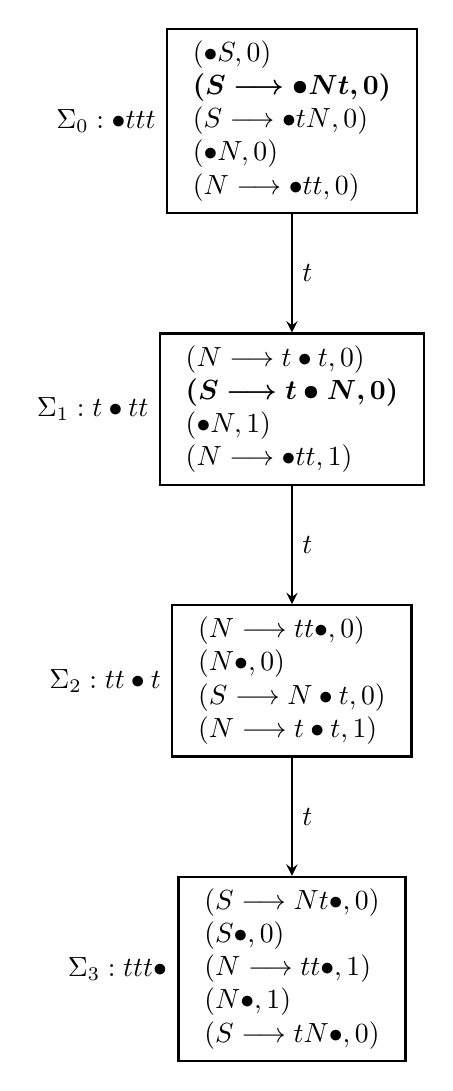
\begin{tikzpicture}[->,>=stealth,node distance = 1.5cm,thick]
\tikzstyle{v}=[rectangle,minimum size=1mm,draw,thick]
\node[v, label=left:$\Sigma_0:\bullet{ttt}$]	(S0)  					   		{\begin{tabular}{l}
  $(\bullet{S}, 0)$\\
  \bm{$(S\longrightarrow{\bullet{Nt}}, 0)$}\\
  $(S\longrightarrow{\bullet{tN}}, 0)$\\
  $(\bullet{N}, 0)$\\
  $(N\longrightarrow{\bullet{tt}}, 0)$\\
 \end{tabular}};
\node[v, label=left:$\Sigma_1:t\bullet{tt}$]	(S1)	[below = of S0]			   		{\begin{tabular}{l}
  $(N\longrightarrow{t\bullet{t}}, 0)$\\
  \bm{$(S\longrightarrow{t\bullet{N}}, 0)$}\\
  $(\bullet{N}, 1)$\\
  $(N\longrightarrow{\bullet{tt}}, 1)$\\
 \end{tabular}};
\node[v, label=left:$\Sigma_2:tt\bullet{t}$]	(S2)	[below = of S1]			   		{\begin{tabular}{l}
  $(N\longrightarrow{tt\bullet}, 0)$\\
  $(N\bullet, 0)$\\
  $(S\longrightarrow{N\bullet{t}}, 0)$\\
  $(N\longrightarrow{t\bullet{t}}, 1)$\\
 \end{tabular}};
\node[v, label=left:$\Sigma_3:ttt\bullet$]	(S3)	[below = of S2]			   		{\begin{tabular}{l}
  $(S\longrightarrow{Nt\bullet}, 0)$\\
  $(S\bullet, 0)$\\
  $(N\longrightarrow{tt\bullet}, 1)$\\
  $(N\bullet, 1)$\\
  $(S\longrightarrow{tN\bullet}, 0)$\\
 \end{tabular}};
\path(S0)		edge	node[right]			{$t$}		(S1)
	 (S1)		edge	node[right]			{$t$}		(S2)
	 (S2)		edge	node[right]			{$t$}		(S3);
\end{tikzpicture}
\caption{Example of Earley Sets for the preceding grammar on string "ttt". Call nodes are in bold.} \label{fig:M2}
\end{center}	
\end{figure}

\section{Earley's Algorithm}
Even though Earley's Algorithm is difficult to understand in the standard context, from the prospective of GFGs, it is just an algorithm that simulates the NGA. For an input string $w$, the algorithm generates a sequence of Earley sets, $\Sigma_0, \Sigma_1, \dots, \Sigma_{|w|}$, in which each set is a set of nodes from the GFG. Each set $\Sigma_i$ is the $\epsilon$-closure of $\Sigma_{i-1}$, that is each node in $\Sigma_i$ is reachable from a node in $\Sigma_{i-1}$ by traversing edges labeled $\epsilon$ in the GFG after traversing a scan edge labeled with the character at position $i$ in string $w$. As its definition, $\Sigma_0$ contains $(\bullet{S})$ and no characters from the string $w$. Intuitively, you can imagine that the characters in $w$ start their numbering at position $1$. 

Recall that at an end node, the NGA should take the return edge corresponding to the call edge it took. This can be handled by associating a tag with each node in the Earley sets. At a high level, these tags differentiate the times at which the start nodes are reached and they propogate this information to the corresponding end nodes. At the end nodes, the tags are consulted to find the appropriate return edge. Thus when a call edge is traversed from a call node to a start node, the start node gets tagged with the number of the Earley Set to which the call and start nodes are added. At an end node, the tag identifies the Earley Set in which the call node resides after which the corresponding return node can be easily identified and tagged with the tag of its call node. All other edges simply copy these tags. We thus have the following theorem.

\textit{Thereom 2}: Let $CFG=(N, T, P, S)$ and let $w$ be an input string. $(S\bullet, 0)\in{\Sigma_{|w|}}$ iff $w$ is part of the language produced by $CFG$.

\textit{Proof}: Please see \cite{bilardi-pingali}.

Figure \ref{fig:M2} displays the Earley Sets on the input string "ttt" giving by the following grammar whose GFG is provided in Figure \ref{fig:M1}.
\begin{align*}
S&\longrightarrow{N \: t \: | \: t \: N} \\
N&\longrightarrow{t \: t}
\end{align*}

\section{Shared Packed Parse Forest (SPPF}
Even though a Shared Packed Parse Forest was the purpose of her algorithm, Dr. Elizabeth Scott only gave it a brief description. Here, we will try to provide a more intuitive understanding of this data structure. First, consider the following ambiguous grammar:$$S \longrightarrow S \: S \: | \: u$$

\begin{figure}
\begin{center}
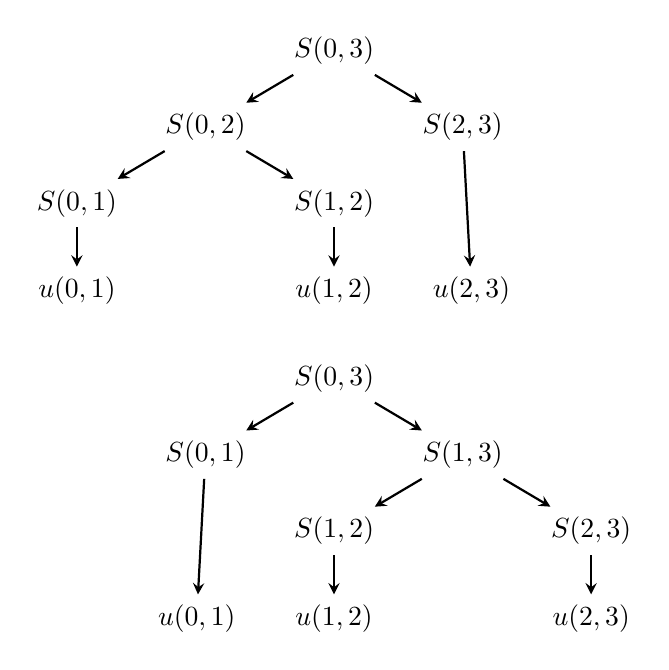
\begin{tikzpicture}[->,>=stealth,node distance = 0.5cm,thick]
\tikzstyle{v}=[]
\node[v]	(S03)	  					   		{$S(0,3)$};
\node[v]	(S02)  	[below left= of S03]		{$S(0,2)$};
\node[v]	(S23)  	[below right= of S03]		{$S(2,3)$};
\node[v]	(S01)  	[below left= of S02]		{$S(0,1)$};
\node[v]	(S12)  	[below right= of S02]		{$S(1,2)$};
\node[v]	(u01)  	[below = of S01]			{$u(0,1)$};
\node[v]	(u12)  	[below = of S12]			{$u(1,2)$};
\node[v]	(u23)  	[right = of u12]			{$u(2,3)$};
\node[v]	(T03)	[below = of u12]  			{$S(0,3)$};
\node[v]	(T01)  	[below left= of T03]		{$S(0,1)$};
\node[v]	(T13)  	[below right= of T03]		{$S(1,3)$};
\node[v]	(T12)  	[below left= of T13]		{$S(1,2)$};
\node[v]	(T23)  	[below right= of T13]		{$S(2,3)$};
\node[v]	(v12)  	[below = of T12]			{$u(1,2)$};
\node[v]	(v01)  	[left = of v12]				{$u(0,1)$};
\node[v]	(v23)  	[below = of T23]			{$u(2,3)$};
\path(S03)		edge	node			{}		(S02)
     (S03)		edge	node			{}		(S23)
     (S02)		edge	node			{}		(S01)
     (S02)		edge	node			{}		(S12)
     (S01)		edge	node			{}		(u01)
     (S12)		edge	node			{}		(u12)
     (S23)		edge	node			{}		(u23)
     (T03)		edge	node			{}		(T01)
     (T03)		edge	node			{}		(T13)
     (T13)		edge	node			{}		(T12)
     (T13)		edge	node			{}		(T23)
     (T01)		edge	node			{}		(v01)
     (T12)		edge	node			{}		(v12)
     (T23)		edge	node			{}		(v23);
\end{tikzpicture}
\caption{The two parse trees of "uuu" for the preceding grammar} \label{fig:M3}
\end{center}	
\end{figure}

Figure \ref{fig:M3} displays the two parse trees of the string "uuu" that is part of the above grammar. The meaning of the numbers at each node are as follows. Giving the string "uuu", number the string as shown:$$0 \quad u \quad 1 \quad u \quad 2 \quad u \quad 3$$ So $u(0,1)$ indicates that the $u$ of interest is between the numbers $0$ and $1$,  $u(1,2)$ indicates that the $u$ of interest is between the numbers $1$ and $2$, and so on. The numbers of the interior nodes are just natural extensions of this pattern.

Let us ignore these numbers for the moment and just consider the most natural way that allows us to share the common subtrees that appear in both parse trees in Figure \ref{fig:M3}. Notice that both subtrees consist of a root node $S$ whose children consist of two other nodes, lets call them $S_l$ and $S_r$ for the moment. The difference between the two parse trees only begins to appear at level $3$ in which we have two alternatives:
\begin{itemize}
\item Either $S_l$ contains two children, $S_m,S_s$ and $S_r$ goes directly to a leaf $u$
\item or $S_l$ goes directly to a leaf $u$ and $S_r$ contains two children, $S_m,S_s$.
\end{itemize}
We can capture this intuitive notion by the \textit{and-or} tree in Figure \ref{fig:M4}, where the subscripts are ignored since they are immaterial. An \textit{and} node represents the action that you consider both children of the node while an \textit{or} node represents the action that you consider one child of the node. However, observe that this tree represents strings other than "uuu". To see this, consider starting at the root node and following its edges to both of its children. Here, you are at two \textit{or} nodes both labeled $S$. Since we are at \textit{or} nodes, we choose a single child for each node. Suppose we choose the leaf children, resulting in the string "uu". To correct this error, we reintroduce the numbers associated with each node and require that only nodes with identical names and numbers can share structure from the tree. Figure \ref{fig:M5} shows our correction.

\begin{figure}
\begin{center}
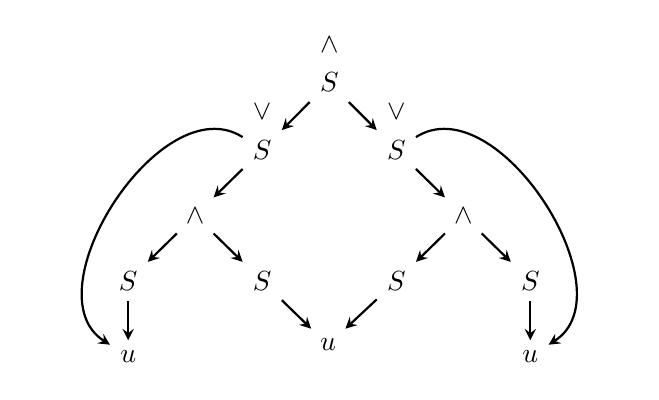
\begin{tikzpicture}[->,>=stealth,node distance = 0.5cm,thick]
\tikzstyle{v}=[]
\node[v, label=$\land$]	(S)	  					   		{$S$};
\node[v, label=$\lor$]	(SL)  	[below left= of S]		{$S$};
\node[v, label=$\lor$]	(SR)  	[below right= of S]		{$S$};
\node[v]	(ALR)  	[below left= of SL]			{$\land$};
\node[v]	(ARL)  	[below right= of SR]			{$\land$};
\node[v]	(SLRL)  [below left= of ALR]	{$S$};
\node[v]	(SLRR)  [below right= of ALR]	{$S$};
\node[v]	(SRLL)  [below left= of ARL]	{$S$};
\node[v]	(SRLR)  [below right= of ARL]	{$S$};
\node[v]	(u01)   [below = of SLRL]		{$u$};
\node[v]	(u12)   [below right= of SLRR]	{$u$};
\node[v]	(u23)   [below = of SRLR]		{$u$};
\path(S)		edge	node			{}		(SL)
	 (S)		edge	node			{}		(SR)
	 (SL)		edge	[bend right = 90]		node			{}		(u01)
	 (SL)		edge	node  			{}		(ALR)
	 (ALR)		edge	node			{}		(SLRL)
	 (ALR)		edge	node			{}		(SLRR)
	 (SR)		edge	[bend left = 90]		node			{}		(u23)
	 (SR)		edge	node  			{}		(ARL)
	 (ARL)		edge	node			{}		(SRLL)
	 (ARL)		edge	node			{}		(SRLR)
	 (SLRL)		edge	node			{}		(u01)
	 (SLRR)		edge	node			{}		(u12)
	 (SRLL)		edge	node			{}		(u12)
	 (SRLR)		edge	node			{}		(u23);
\end{tikzpicture}
\caption{The and-or tree representation of the two parse trees in Figure \ref{fig:M3}.} \label{fig:M4}
\end{center}	
\end{figure}

\begin{figure}
\begin{center}
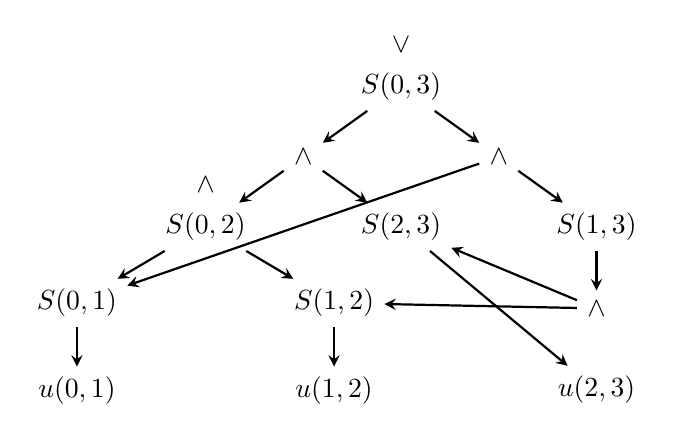
\begin{tikzpicture}[->,>=stealth,node distance = 0.5cm,thick]
\tikzstyle{v}=[]
\node[v, label=$\lor$]	(S03)	  					   		{$S(0,3)$};
\node[v]	(AL)	[below left= of S03]   		{$\land$};
\node[v]	(AR)	[below right= of S03]   	{$\land$};
\node[v ,label=$\land$]	(S02)  	[below left= of AL]			{$S(0,2)$};
\node[v]	(S23)  	[below right= of AL]		{$S(2,3)$};
\node[v]	(S13)	[below right= of AR]   		{$S(1,3)$};
\node[v]	(ARR)	[below = of S13]   			{$\land$};
\node[v]	(S01)  	[below left= of S02]		{$S(0,1)$};
\node[v]	(S12)  	[below right= of S02]		{$S(1,2)$};
\node[v]	(u01)  	[below = of S01]			{$u(0,1)$};
\node[v]	(u12)  	[below = of S12]			{$u(1,2)$};
\node[v]	(u23)  	[below = of ARR]			{$u(2,3)$};

\path(S03)		edge	node			{}		(AL)
	 (S03)		edge	node			{}		(AR)
	 (AL)		edge	node			{}		(S02)
	 (AL)		edge	node			{}		(S23)
	 (AR)		edge	node			{}		(S01)
	 (AR)		edge	node			{}		(S13)
	 (S02)		edge	node			{}		(S01)
	 (S02)		edge	node			{}		(S12)
	 (S13)		edge	node			{}		(ARR)
	 (ARR)		edge	node			{}		(S12)
	 (ARR)		edge	node			{}		(S23)
	 (S01)		edge	node			{}		(u01)
	 (S12)		edge	node			{}		(u12)
	 (S23)		edge	node			{}		(u23);
\end{tikzpicture}
\caption{The SPPF representation of the two parse trees in Figure \ref{fig:M3}.} \label{fig:M5}
\end{center}	
\end{figure}

The data structure we have constructed is what Dr. Elizabeth Scott calls a Shared Packed Parse Forest (SPPF). For sake of completeness, we present her definition. Note that in her definition, her \textit{packed} nodes are our nameless \textit{and} nodes.

\textit{Definition}: A \textit{Shared Packed Parse Forest (SPPF)} is a representation that reduces the space used to represent multiple parse trees of an ambiguous string. Nodes are are named $(x,j,i)$, when node $x$ matches substring $a_{j+1}\dots{a_i}$. Nodes which contain the same sub-tree are shared and nodes which represent the same substring for nonterminals with different parse trees are packed. 

\section{Earley's Parser}
Dr. Elizabeth Scott presented two algorithms that constructed SPPFs. The first algorithm decorates the Earley Sets with pointers as they are being constructed and subsequently walks through the sets using these pointers to create the SPPF. The second algorithm creates the SPPF as the Earley Sets are being constructed. We choose to discuss this second algorithm since the SPPF it produces is much cleaner than the one produced by the first algorithm. This is because some of the intermediate nodes created by the first algorithm are ignored by the second algorithm. The omission of these nodes not only decreases the size of the SPPF but also allows for a more efficient parser. 
 
We will now discuss her algorithm which we will subsequently call the parser. At a high level, the parser loops through the characters in the input string, $a[1..n]$ and for each position $i$, it creates the Earley Set $\Sigma_{i-1}$ and connects the leaf node representing $a_i$ to the rest of the SPPF. This requires a modification the elements in the Earley Sets. Recall from Section 3 that each element in an Earley Set is a tuple $(n_g, t)$, where $n_g$ is a node in the GFG and $t$ is the tag associated with that node. We simply extend this tuple to include one more field, $(n_g, t, n_s)$, where $n_s$ is the associated SPPF node. Recall from section 4 that $n_s = (x,j,i)$ when node $x$ matches substring $a_{j+1}\dots{a_i}$. If an element in the Earley Set does not have an associated SPPF node, then $n_s$ is simply null.

As we compute the $\epsilon$-closure over the GFG, we maintain two auxilliary sets, $Q$ and $R$. $Q$ contains the scan nodes we encountered in the current iteration while $R$ contains the other nodes. Intuitively $R$ is a worklist that contains the nodes that still need to be processed in the current iteration and $Q$ are the nodes that need to be processed to initialize the next Earley Set. Keep in mind that the whole point of an SPPF is to faciliate structure sharing, so when a node is desired we first check if it already exists. We maintain a cache, $V$, of nodes that are created in the current iteration for that purpose.

Special care must be taken for Earley elements of the form $(n_g,i,n_s)$ when $n_g$ is an exit node in $\Sigma_i$. This indicates that no scan edges were traversed between the start node and the exit node, meaning we have encountered an $\epsilon$-production. Therefore the corresponding Earley element representing the call node must exist in $\Sigma_i$. The catch is that the Earley element representing the call node could be created after the the Earley element representing the exit node have already been processed. To this end, we maintain a set $H$ in which tuples of the form $(n_g,n_s)$ are added after $(n_g,i,n_s)\in{\Sigma_i}$ have been processed. Subsequently, when an Earley element representing a call node is processed, $H$ is consulted. 

We now present her algorithm:
\begin{algorithm}[!h]\label{alg:EP}
	\caption{EarleyParser}
	\textbf{Input:} 
	\begin{itemize}
	\item[] A grammar $\Gamma = (N,T,P,S)$
	\item[] A string $a[1..n]$
	\end{itemize}
	\textbf{Output:} 
	\begin{itemize}
	\item[] The corresponding Earley Sets and SPPF if $G$ produces $a$
	\end{itemize}
	\textbf{begin}
	
	Initialize $\Sigma_0\dots{\Sigma_n}, R, Q', V = \emptyset$ \;
	Begin at $(\bullet{S})$ in the GFG and compute the $\epsilon$-closure \;
	\quad Let $n$ denote the reachable nodes that are not scan nodes \; 
	\quad Add $(n,0,null)$ to $\Sigma_0$ \;
	\quad Let $s$ denote the reachable nodes that are scan nodes \; 
	\quad Add $(s,0,null)$ to $Q'$ \;
	\For{\text{$0\leq{i\leq{n}}$}}
	{
	Set $R=\Sigma_i$, $Q=Q'$ \;
	Initialize $H,Q'=\emptyset$ \;
	$Worklist(R,Q,H,V)$ \;
	Set $V=\emptyset$ \;
	Create a node $v=(a_{i+1},i,i+1)$ \;
	\While {\text{$Q\neq{\emptyset}$}}
	{
	Remove an element $q=(n_g,t,n_s)$ from $Q$ \;
	$n_g$ is a scan node so there is an edge $(n_g,n'_g)$ in the GFG \;
    $y=MakeNode(n'_g,t,i+1,n_s,v,V)$ \;
    Let $n$ denote the reachable nodes that are not scan nodes \;
    Add $(n'_g,t,y)$ to $\Sigma_{i+1}$ \;
    Let $s$ denote the reachable nodes that are scan nodes \;
    Add $(n'_g,t,y)$ to $Q'$ \;
    }
    }
    Let $s_e$ by the end node for the Start Symbol \;
    \eIf {\text{$(s_e,0,n_s)\in{\Sigma_n}$}}{\Return $n_s$}{fail} 
    \textbf{end}
\end{algorithm}

\begin{algorithm}[!h]\label{alg:W}
	\caption{Worklist}
	\textbf{Input:} 
	\begin{itemize}
	\item[] $R$, the nodes that still need to be processed in the current iteration
	\item[] $Q$, the nodes that need to be processed to initialize the next Earley Set 
	\item[] $H$, the call nodes to epsilon productions
	\item[] $V$, cache of nodes created during the current iteration
	\end{itemize}
	\textbf{begin}
	
	\While {\text{$R\neq{\emptyset}$}}
	{
	Remove an element $r=(n_g,t,n_s)$ from $R$ \;
	\If {\text{$r$ represents a call node for a nonterminal $C$}}
	{
	Compute the $\epsilon$-closure \;
	\quad Let $n$ denote the reachable nodes that are not scan nodes \;
	\quad Add $(n,i,null)$ to $\Sigma_i$ and $R$ if they are not in them already \;
	\quad Let $s$ denote the reachable nodes that are scan nodes \; 
	\quad Add $(s,i,null)$ to $Q$ \;
    Let $n_e$ be the exit node corresponding to $n_g$ \;
    \If {\text{$(n_e,n_s)\in{H}$}}
    {
    Let $n_h$ be the return node corresponding to $n_g$ \;
	$y=MakeNode(n_h,t,i,n_s,null,V)$ \; 
	Let $n$ denote the reachable nodes that are not scan nodes \;
    Add $(n,t,y)$ to $\Sigma_i$ and $R$ if they are not in them already \;
    Let $s$ denote the reachable nodes that are scan nodes \;
    Add $(s,t,y)$ to $Q$ \;
    }
	}
	\If {\text{$r$ represents an exit node for a nonterminal $D$}}
	{
	\If {\text{$n_s$ is null}}
	{
	Create a node $v=(n_g,i,i)$ if it is not already in $V$ \;
	set $n_s = v$ \;
	Make $\epsilon$ a child of $n_s$ if it isn't already \;
	}
	\If {$t == i$}{add $(n_g,n_s)$ to $H$}
	\For {\text{$\sigma{\in{\Sigma_t}}$ representing call nodes, $n_c$, corresponding to $n_g$}}
	{
	Let $\sigma = (n_c,t',n'_s)$ \;
	Let $n_h$ be the return nodes corresponding to $n_c$ \;
    $y=MakeNode(n_h,t',i,n'_s,n_s,V)$ \;
    Let $n$ denote the reachable nodes that are not scan nodes \;
    Add $(n,t',y)$ to $\Sigma_i$ and $R$ if they are not in them already \; 
    Let $s$ denote the reachable nodes that are scan nodes \;
    Add $(s,t',y)$ to $Q$ \;
	}
	}
	}
	\textbf{end}
\end{algorithm}

\begin{algorithm}[!h]\label{alg:MN}
	\caption{MakeNode}
	\textbf{Input:} 
	\begin{itemize}
	\item[] $n_g$, a GFG node
	\item[] $j,i$ substring indices where $j\leq{i}$
	\item[] $w,v$, SPPF nodes
	\item[] $V$, cache of nodes created during the current iteration
	\end{itemize}
	\textbf{Output:} 
	\begin{itemize}
	\item[] $y$, a new SPPF node
	\end{itemize}
	\textbf{begin}
	
	\eIf {\text{$n_g$ is an exit node of a nonterminal $B$}}{set $s=B$}{set $s=n_g$}
	\eIf {\text{$n_g$ is the second scan node and not an exit node}}{set $y=v$}
	{
	Create a node $y=(s,j,i)$ if it is not already in $V$ and add it to $V$ \;
	\If {\text{$w$ is null}}{make $v$ a child of $y$ if it isn't already}
    \If {\text{$w$ is not null}}{make $w$ and $v$ children of $y$ if they aren't already}
	}
	\Return $y$ \;
	\textbf{end}
\end{algorithm}

\section{Implementation}
We have coded up a faithful implementation of the Earley Parser using Python 2.7.6. Just like how the conceptual components of this paper have been broken up into 4 sections, we have broken up our code base into into 4 logical units in which each unit is a class that handles one major task. We will discuss the following in turn:
\begin{itemize}
\item GrammarFlowGraph.py
\item SigmaSet.py
\item SharedPackedParseForest.py
\item earlyParser.py
\end{itemize}

\subsection{GrammarFlowGraph.py}
Here contains the logic that handles GFG construction. There are 3 classes contained within this file: Node, Edge, and GFG. 

Each Node has a name, the reference to its endNode, and a set of outgoing edges. An endNode of a Node $u$ is simply a Node that logically follows $u$ in its production. For instance, if $u=(A\longrightarrow{\bullet{BC}})$ then the endNode of u will be $(A\longrightarrow{B\bullet{C}})$. Finally we reserve a special field, callNode, for a Node's call node if it has one.

Each Edge has a reference to its two endpoints and a weight, which is the label associated with it.

Each GFG a contains a set of Nodes, of which a special field, startNode, is reserved for a GFG's start node. When GFG's constructor is called, the entire graph is built from a grammar file. The GFG is built by processing each line of the grammar file out of which a grammar production is extracted and the nonterminals added to the GFG if they do not already exist in the graph. We then walk through the production to create the appropriate Nodes and Edges in the GFG, taking special care when encountering nonterminals so that we add their corresponding call and return edges.

\subsection{SigmaSet.py}

Here contains the logic that handles the interface for Earley Sets. There are 2 classes contained within this file: sigmaSetItem and SSet.

Each sigmaSetItem consists of a node of the GFG, a counter, and a sppfNode. 

Each SSet contains an id, a set callSet of call nodes, a pathSet that corresponds to the set Q in Algorithm \ref{alg:W}, and nodeSet that contains the rest of the GFG nodes.  

\subsection{SharedPackedParseForest.py}

Here contains the logic that handles the interface for a Shared Packed Parse Forest. There are 4 classes contained within this file: NodeType, Node, Edge, and SPPF.

NodeType is simply an object class for a Node to distinguish whether it is an \textit{and} node, an \textit{or} node, or a leaf node.

Each Node has a name, a list of outgoing edges and a nodeType. In addition a Node keeps tracks of the startPos and the endPos which correspond to the indices of the substring it matches. 

Each Edge has a reference to its two endpoints. 

Each SPPF contains a set of Nodes and their associated names. We make note here that Algorithm \ref{alg:MN} belongs to this class.

\subsection{earleyParser.py}

Here contains the logic that handles the parser. There is 1 class contained within this file: Parser.

Each Parser constructs a GFG, has a list of sigmaSets, and initializes an SPPF. When the Parser's constructor is called, the string file is parsed using the GFG. We make note that Algorithm \ref{alg:EP} gets invoked here.

\section{Results and Future Work}

Feeding the grammar $$S\longrightarrow{S\:{S\:{|\:{b}}}}$$ along with the string $$"b\;{b\:{b}}"$$ into \textit{earleyParser.py} produces the output shown in Figure \ref{fig:M6}. The graph associated is depicted in Figure \ref{fig:M7}. Notice that the resulting SPPF produced by our implementation contains extra \textit{and} nodes. Although these extra nodes do not negatively effect the correctness, removing them using some post-processing would result in a much cleaner representation.

Another aspect of our implementation that could benefit from further development pertains to the source code itself. Notice that in the previous section we have two separate classes for Nodes and two separate classes for Edges. This repetition is not entirely intentional since the construction of our code base is inherently bottom-up. The next logical step would have been to create an abstract class for a Node, Edge and Graph then subsequently have the classes in \textit{GrammarFlowGraph.py} and \textit{SharedPackedParseForest.py} inherit from these base classes.

During the coding process, we tried our best to follow good object-oriented techniques so that the code base could be potentially maintained by others who are interested in our work. However, there are aspects of the source code that can benefit greatly from refactoring. The logic most central to our implementation such as building the GFG and construction the SPPF are within the methods \textit{GFG.build()} and \textit{Parser.parse()} respectively. Even though \textit{Parser.parse()} calls \textit{Parser.analyzeSigmaSet()} to handle Algorithm \ref{alg:W}, these methods are extremely large and span more than 100 lines of code. Thus it would greatly benefit others if methods such as these are broken up and extracted into many smaller methods that perform the same task.

We have tested our implementation against all the examples given in Dr. Scott's paper, \cite{scott}, and we can successfully produce the expected SPPFs. However, these grammars are relatively simple so it would be interesting to see how our parser scales to more realistic grammars such as the one for the C programming language.  This is the next logical step for this project.

The most important insight we would like to be gleaned from our project is the idea that the threshold to understanding is not a property related the difficulty of the concept itself but rather it is a characteristic of the way in which that concept is presented. Earley's Algorithm is difficult to understand in terms of grammar rules and production but is significantly simplified in terms of  finding paths through a graph. Similarly, Dr. Scott's algorithm can benefit from this shift in perspective.

\begin{figure}
\begin{center}
\begin{align*}
&Nodes: \\
&<S03,0,3,OR> \\
&<S02,0,2,OR> \\
&<AND[u'b']01,0,1,AND> \\
&<ANDS01S12,0,2,AND> \\
&<AND[u'b']23,2,3,AND> \\
&<ANDS12S23,1,3,AND> \\
&<[u'b']12,1,2,LEAF> \\
&<[u'b']23,2,3,LEAF> \\
&<S23,2,3,OR> \\
&<S01,0,1,OR> \\
&<ANDS02S23,0,3,AND> \\
&<AND[u'b']12,1,2,AND> \\
&<S13,1,3,OR> \\
&<ANDS01S13,0,3,AND> \\
&<S12,1,2,OR> \\
&<[u'b']01,0,1,LEAF> \\
\\
&Edges: \\
&<ANDS02S23,0,3,AND>\longrightarrow<S23,2,3,OR> \\
&<ANDS01S13,0,3,AND>\longrightarrow<S01,0,1,OR> \\
&<ANDS12S23,1,3,AND>\longrightarrow<S12,1,2,OR> \\
&<ANDS01S12,0,2,AND>\longrightarrow<S12,1,2,OR> \\
&<S23,2,3,OR>\longrightarrow<AND[u'b']23,2,3,AND> \\
&<ANDS12S23,1,3,AND>\longrightarrow<S23,2,3,OR> \\
&<AND[u'b']23,2,3,AND>\longrightarrow<[u'b']23,2,3,LEAF> \\
&<S01,0,1,OR>\longrightarrow<AND[u'b']01,0,1,AND> \\
&<S13,1,3,OR>\longrightarrow<ANDS12S23,1,3,AND> \\
&<S12,1,2,OR>\longrightarrow<AND[u'b']12,1,2,AND> \\
&<ANDS01S12,0,2,AND>\longrightarrow<S01,0,1,OR> \\
&<AND[u'b']12,1,2,AND>\longrightarrow<[u'b']12,1,2,LEAF>  \\
&<AND[u'b']01,0,1,AND>\longrightarrow<[u'b']01,0,1,LEAF> \\
&<ANDS01S13,0,3,AND>\longrightarrow<S13,1,3,OR> \\
&<S03,0,3,OR>\longrightarrow<ANDS01S13,0,3,AND> \\
&<ANDS02S23,0,3,AND>\longrightarrow<S02,0,2,OR> \\
&<S02,0,2,OR>\longrightarrow<ANDS01S12,0,2,AND> \\
&<S03,0,3,OR>\longrightarrow<ANDS02S23,0,3,AND> \\
\end{align*}
\caption{The output of our earleyParser when given $S\longrightarrow{S\:{S\:{|\:{b}}}}$ and the string "b b b".} \label{fig:M6}
\end{center}
\end{figure}

\begin{figure}
\begin{center}
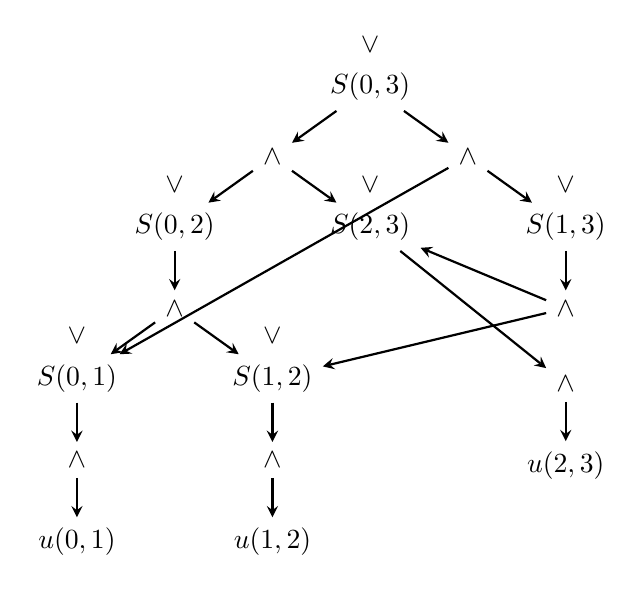
\begin{tikzpicture}[->,>=stealth,node distance = 0.5cm,thick]
\tikzstyle{v}=[]
\node[v, label=$\lor$]	(S03)	  					   		{$S(0,3)$};
\node[v]	(AL)	[below left= of S03]   		{$\land$};
\node[v]	(AR)	[below right= of S03]   	{$\land$};
\node[v, label=$\lor$]	(S02)  	[below left= of AL]			{$S(0,2)$};
\node[v]	(A02)  	[below = of S02]			{$\land$};
\node[v, label=$\lor$]	(S23)  	[below right= of AL]		{$S(2,3)$};
\node[v, label=$\lor$]	(S13)	[below right= of AR]   		{$S(1,3)$};
\node[v]	(ARR)	[below = of S13]   			{$\land$};
\node[v, label=$\lor$]	(S01)  	[below left= of A02]		{$S(0,1)$};
\node[v]	(A01)  	[below = of S01]			{$\land$};
\node[v, label=$\lor$]	(S12)  	[below right= of A02]		{$S(1,2)$};
\node[v]	(A12)  	[below = of S12]			{$\land$};
\node[v]	(u01)  	[below = of A01]			{$u(0,1)$};
\node[v]	(u12)  	[below = of A12]			{$u(1,2)$};
\node[v]	(A23)  	[below = of ARR]			{$\land$};
\node[v]	(u23)  	[below = of A23]			{$u(2,3)$};

\path(S03)		edge	node			{}		(AL)
	 (S03)		edge	node			{}		(AR)
	 (AL)		edge	node			{}		(S02)
	 (AL)		edge	node			{}		(S23)
	 (AR)		edge	node			{}		(S01)
	 (AR)		edge	node			{}		(S13)
	 (S02)		edge	node			{}		(A02)
	 (A02)		edge	node			{}		(S01)
	 (A02)		edge	node			{}		(S12)
	 (S13)		edge	node			{}		(ARR)
	 (ARR)		edge	node			{}		(S12)
	 (ARR)		edge	node			{}		(S23)
	 (S01)		edge	node			{}		(A01)
	 (A01)		edge	node			{}		(u01)
	 (S12)		edge	node			{}		(A12)
	 (A12)		edge	node			{}		(u12)
	 (S23)		edge	node			{}		(A23)
	 (A23)		edge	node			{}		(u23);
\end{tikzpicture}
\caption{The graphical representation of the output in Figure \ref{fig:M6}.} \label{fig:M7}
\end{center}	
\end{figure}

\acks
We would like to thank Dr. Keshav Pingali for his guidance on this project. We would also like to thank Sepideh Maleki for helping us understand Scott's algorithm.

% We recommend abbrvnat bibliography style.

\bibliographystyle{abbrvnat}

% The bibliography should be embedded for final submission.

\begin{thebibliography}{}
\softraggedright

\bibitem[Bilardi and Pingali(2012)]{bilardi-pingali}
Gianfranco Bilardi, and Keshav Pingali. Parsing with Pictures. UTCS Tech Reports, 2012. This is a full TECHREPORT entry.

\bibitem[Scott(2008)]{scott}
Elizabeth Scott. SPPF-Style Parsing From Earley Recognisers. \textit{Electronic Notes in Theoretical Computer Science}, 203(53-67), 2008. This is a full ARTICLE entry.

\end{thebibliography}


\end{document}

%                       Revision History
%                       -------- -------
%  Date         Person  Ver.    Change
%  ----         ------  ----    ------

%  2013.06.29   TU      0.1--4  comments on permission/copyright notices

